\documentclass[10pt,dvipsnames,hyperref={colorlinks=false}]{beamer}

% for graphic support
\usepackage{graphicx}
\graphicspath{{./figures/}}

% to put text over picture
\usepackage{overpic}
\usepackage{tikz}
\usetikzlibrary{decorations.pathreplacing,calc,tikzmark}

% for tables
\usepackage{tabularx, multirow, makecell, booktabs}
\usepackage{enumitem}
\setlist[itemize]{label=$\bullet$}

% for math support
\usepackage{amsmath,amssymb}
\usefonttheme{professionalfonts}
\setlength{\jot}{5pt}
\usepackage{siunitx}
\usepackage[version=4]{mhchem}

% for code
\usepackage{minted}
\definecolor{codebg}{gray}{0.95}
\setminted[vim]{
    frame=lines,
    framesep=2mm,
    baselinestretch=1.2,
    bgcolor=codebg,
    fontsize=\footnotesize,
    breaklines
    % linenos
}
\setminted[python]{
    frame=lines,
    framesep=2mm,
    baselinestretch=1.2,
    bgcolor=codebg,
    fontsize=\footnotesize,
    breaklines
    % linenos
}

\usepackage[backend=biber, style=authoryear-icomp]{biblatex}
\addbibresource{pdr_references.bib}
%
%  These Macros are taken from the AAS TeX macro package version 5.2
%  and are compatible with the macros in the A&A document class
%  version 7.0
%  Include this file in your LaTeX source only if you are not using
%  the AAS TeX macro package or the A&A document class and need to
%  resolve the macro definitions in the TeX/BibTeX entries returned by
%  the ADS abstract service.
%
%  If you plan not to use this file to resolve the journal macros
%  rather than the whole AAS TeX macro package, you should save the
%  file as ``aas_macros.sty'' and then include it in your LaTeX paper
%  by using a construct such as:
%	\documentstyle[11pt,aas_macros]{article}
%
%  For more information on the AASTeX and A&A packages, please see:
%       http://journals.aas.org/authors/aastex.html	
%       ftp://ftp.edpsciences.org/pub/aa/readme.html
%  For more information about ADS abstract server, please see:
%       http://adsabs.harvard.edu/ads_abstracts.html
%

% Abbreviations for journals.  The object here is to provide authors
% with convenient shorthands for the most "popular" (often-cited)
% journals; the author can use these markup tags without being concerned
% about the exact form of the journal abbreviation, or its formatting.
% It is up to the keeper of the macros to make sure the macros expand
% to the proper text.  If macro package writers agree to all use the
% same TeX command name, authors only have to remember one thing, and
% the style file will take care of editorial preferences.  This also
% applies when a single journal decides to revamp its abbreviating
% scheme, as happened with the ApJ (Abt 1991).

\makeatletter
\let\jnl@style=\rm
\def\ref@jnl#1{{\jnl@style#1}}

\def\aj{\ref@jnl{AJ}}                   % Astronomical Journal
\def\actaa{\ref@jnl{Acta Astron.}}      % Acta Astronomica
\def\araa{\ref@jnl{ARA\&A}}             % Annual Review of Astron and Astrophys
\def\apj{\ref@jnl{ApJ}}                 % Astrophysical Journal
\def\apjl{\ref@jnl{ApJ}}                % Astrophysical Journal, Letters
\def\apjs{\ref@jnl{ApJS}}               % Astrophysical Journal, Supplement
\def\ao{\ref@jnl{Appl.~Opt.}}           % Applied Optics
\def\apss{\ref@jnl{Ap\&SS}}             % Astrophysics and Space Science
\def\aap{\ref@jnl{A\&A}}                % Astronomy and Astrophysics
\def\aapr{\ref@jnl{A\&A~Rev.}}          % Astronomy and Astrophysics Reviews
\def\aaps{\ref@jnl{A\&AS}}              % Astronomy and Astrophysics, Supplement
\def\azh{\ref@jnl{AZh}}                 % Astronomicheskii Zhurnal
\def\baas{\ref@jnl{BAAS}}               % Bulletin of the AAS
\def\bac{\ref@jnl{Bull. astr. Inst. Czechosl.}}
                % Bulletin of the Astronomical Institutes of Czechoslovakia 
\def\caa{\ref@jnl{Chinese Astron. Astrophys.}}
                % Chinese Astronomy and Astrophysics
\def\cjaa{\ref@jnl{Chinese J. Astron. Astrophys.}}
                % Chinese Journal of Astronomy and Astrophysics
\def\icarus{\ref@jnl{Icarus}}           % Icarus
\def\jcap{\ref@jnl{J. Cosmology Astropart. Phys.}}
                % Journal of Cosmology and Astroparticle Physics
\def\jrasc{\ref@jnl{JRASC}}             % Journal of the RAS of Canada
\def\memras{\ref@jnl{MmRAS}}            % Memoirs of the RAS
\def\mnras{\ref@jnl{MNRAS}}             % Monthly Notices of the RAS
\def\na{\ref@jnl{New A}}                % New Astronomy
\def\nar{\ref@jnl{New A Rev.}}          % New Astronomy Review
\def\pra{\ref@jnl{Phys.~Rev.~A}}        % Physical Review A: General Physics
\def\prb{\ref@jnl{Phys.~Rev.~B}}        % Physical Review B: Solid State
\def\prc{\ref@jnl{Phys.~Rev.~C}}        % Physical Review C
\def\prd{\ref@jnl{Phys.~Rev.~D}}        % Physical Review D
\def\pre{\ref@jnl{Phys.~Rev.~E}}        % Physical Review E
\def\prl{\ref@jnl{Phys.~Rev.~Lett.}}    % Physical Review Letters
\def\pasa{\ref@jnl{PASA}}               % Publications of the Astron. Soc. of Australia
\def\pasp{\ref@jnl{PASP}}               % Publications of the ASP
\def\pasj{\ref@jnl{PASJ}}               % Publications of the ASJ
\def\rmxaa{\ref@jnl{Rev. Mexicana Astron. Astrofis.}}%
                % Revista Mexicana de Astronomia y Astrofisica
\def\qjras{\ref@jnl{QJRAS}}             % Quarterly Journal of the RAS
\def\skytel{\ref@jnl{S\&T}}             % Sky and Telescope
\def\solphys{\ref@jnl{Sol.~Phys.}}      % Solar Physics
\def\sovast{\ref@jnl{Soviet~Ast.}}      % Soviet Astronomy
\def\ssr{\ref@jnl{Space~Sci.~Rev.}}     % Space Science Reviews
\def\zap{\ref@jnl{ZAp}}                 % Zeitschrift fuer Astrophysik
\def\nat{\ref@jnl{Nature}}              % Nature
\def\iaucirc{\ref@jnl{IAU~Circ.}}       % IAU Cirulars
\def\aplett{\ref@jnl{Astrophys.~Lett.}} % Astrophysics Letters
\def\apspr{\ref@jnl{Astrophys.~Space~Phys.~Res.}}
                % Astrophysics Space Physics Research
\def\bain{\ref@jnl{Bull.~Astron.~Inst.~Netherlands}} 
                % Bulletin Astronomical Institute of the Netherlands
\def\fcp{\ref@jnl{Fund.~Cosmic~Phys.}}  % Fundamental Cosmic Physics
\def\gca{\ref@jnl{Geochim.~Cosmochim.~Acta}}   % Geochimica Cosmochimica Acta
\def\grl{\ref@jnl{Geophys.~Res.~Lett.}} % Geophysics Research Letters
\def\jcp{\ref@jnl{J.~Chem.~Phys.}}      % Journal of Chemical Physics
\def\jgr{\ref@jnl{J.~Geophys.~Res.}}    % Journal of Geophysics Research
\def\jqsrt{\ref@jnl{J.~Quant.~Spec.~Radiat.~Transf.}}
                % Journal of Quantitiative Spectroscopy and Radiative Transfer
\def\memsai{\ref@jnl{Mem.~Soc.~Astron.~Italiana}}
                % Mem. Societa Astronomica Italiana
\def\nphysa{\ref@jnl{Nucl.~Phys.~A}}   % Nuclear Physics A
\def\physrep{\ref@jnl{Phys.~Rep.}}   % Physics Reports
\def\physscr{\ref@jnl{Phys.~Scr}}   % Physica Scripta
\def\planss{\ref@jnl{Planet.~Space~Sci.}}   % Planetary Space Science
\def\procspie{\ref@jnl{Proc.~SPIE}}   % Proceedings of the SPIE

\let\astap=\aap
\let\apjlett=\apjl
\let\apjsupp=\apjs
\let\applopt=\ao
\makeatother

% PSL theme color
\definecolor{PSL}{RGB}{30, 70, 151}
\definecolor{PSL_shade}{RGB}{113, 145, 209}
\definecolor{PSL_dark}{RGB}{4, 41, 117}

% themes
\usetheme{AnnArbor}
\usecolortheme{seahorse}

\setbeamercolor{palette primary}{bg=PSL, fg=white}
\setbeamercolor{palette secondary}{bg=PSL_dark, fg=white}
\setbeamercolor{palette tertiary}{bg=PSL_shade, fg=white}
\setbeamercolor{palette quaternary}{bg=black, fg=white}
\setbeamercolor{palette sidebar primary}{fg=black}

\setbeamercolor{titlelike}{bg=PSL_dark,fg=black}
\setbeamercolor{frametitle}{bg=gray!10!white}
\setbeamercolor{frametitle right}{bg=gray!60!white}

\setbeamercolor{block title}{bg=PSL_dark,fg=white}
\setbeamercolor{block body}{bg=PSL_shade!40!white}

\setbeamertemplate{sections/subsections in toc}[circle]
\addtobeamertemplate{section in toc}{\vskip1em}{}
\setbeamercolor{section in toc}{fg=black}
\setbeamercolor{subsection in toc}{fg=black}

\setbeamertemplate{itemize item}[circle]
\setbeamertemplate{itemize subitem}[circle]
\setbeamertemplate{itemize subsubitem}[circle]

\setbeamercolor{itemize item}{fg=black}
\setbeamercolor{itemize subitem}{fg=black}
\setbeamercolor{itemize subsubitem}{fg=black}

\defbeamertemplate*{title page}{customized}[1][]
{
    \inserttitlegraphic\hfill
    \vfill
    \begin{centering}
        \begin{beamercolorbox}[rounded=true,shadow=true,sep=20pt,center]{title}
          \parbox{.88\textwidth}{\centering\color{white}\usebeamerfont{title}\inserttitle}
        \end{beamercolorbox}%
    \end{centering}
    \vfill
    \hspace{2em}
    \begin{minipage}[t]{.4\textwidth}
        \begin{flushleft}
            Student\\[0.2em]
            Ducheng Lu   
        \end{flushleft}
    \end{minipage}
    \begin{minipage}[t]{.48\textwidth}
        \begin{flushright}
            Supervisors\\[0.2em]
            Franck Le Petit (LERMA)\\
            Emeric Bron (LERMA)\\[2em]
            Jan 2025
        \end{flushright}
    \end{minipage}
}

% formatting 
\setlength{\leftmargin}{0.5cm}
\setlength{\leftmargini}{0.75cm}
\setlength{\leftmarginii}{1cm}

% for backup slides
\newcommand{\backupbegin}{
   \newcounter{finalframe}
   \setcounter{finalframe}{\value{framenumber}}
}
\newcommand{\backupend}{
   \setcounter{framenumber}{\value{finalframe}}
}

%%%%% define your own command %%%%%
\newcommand{\mr}[1]{\mathrm{#1}}
\newcommand{\dd}[1]{\mathrm{d}#1}
\newcommand{\lfird}[2][]{\mathrm{d}#1/\mathrm{d}#2} 
\newcommand{\fird}[2][]{\frac{\mathrm{d}#1}{\mathrm{d}#2}} 
\newcommand{\secd}[2][]{\frac{\mathrm{d}^2#1}{\mathrm{d}#2^2}}
\newcommand{\pfird}[2][]{\frac{\partial#1}{\partial#2}} 
\newcommand{\pfirdat}[3][1]{\left(\frac{\partial#1}{\partial#2}\right)_{\!\!\!#3}} 
\newcommand{\mdpdr}{\mintinline{latex}{MeudonPDR}}
% \newcommand{\qt}[1]{\textcolor{red}{#1}}
\newcommand{\qt}[1]{}

\title[Spherical Wrapper for \mdpdr{}]{Explaining Spatial Profiles of Line Emission in the Horsehead Nebula Using Cloud Surface Curvature}
\titlegraphic{
\includegraphics[width=.5\textwidth]{Observatoire_de_Paris-CoMarquageLERMA-RGB-Noir_sideral.pdf}}
\institute[Observatoire-PSL]{Observatoire-PSL}
\author{Ducheng LU}
\date{Jan 2025}


\begin{document}

\setlength{\abovedisplayskip}{3pt}
\setlength{\belowdisplayskip}{3pt}
\setlength{\abovedisplayshortskip}{3pt}
\setlength{\belowdisplayshortskip}{3pt}

\begin{frame}
    \titlepage
\end{frame}

\section{Introduction}
\subsection{Photodissociation Regions (PDRs)}
% \begin{frame}[t]{Photodissociation Regions (PDRs)}
%     Interstellar medium (ISM): gas and dust between stars in galaxies
%     \begin{itemize}
%         \item \(\sim10\%\) of the total baryonic mass
%         \item main site of star formation
%     \end{itemize}
%     PDR: regions of \textbf{neutral gas} in the ISM where\par\hskip1em \textbf{far-ultraviolet radiation dominates the chemical and heating processes}
%     \begin{columns}[T]
%         \begin{column}{.4\textwidth}
%             \begin{itemize}
%                 \item Heating: \par photoelectric effect\qt{on small grains and PAHs}, cosmic rays
%                 \item Cooling: \par line emission
%             \end{itemize}
%             IR and line emission\par
%             $\Rightarrow$ physical conditions in PDRs
%         \end{column}
%         \begin{column}{.6\textwidth}
%             \begin{overpic}[width=\textwidth]{PDRScheme.png}
%                 \put(21, 0){\begin{tikzpicture}[overlay]
%                     \draw[->, thick] (0, 0) -- (5, 0) node[above left, xshift=1.5em]{\small depth};
%                 \end{tikzpicture}}
%                 \put(70, -5){\scriptsize Credit: Tielens 2005}
%             \end{overpic}
%         \end{column}
%     \end{columns}
% \end{frame}

\begin{frame}[t]{Photodissociation Regions (PDRs)}
    Interstellar medium (ISM): gas and dust between stars in galaxies
    \begin{columns}
        \begin{column}{.58\textwidth}
            \begin{itemize}
                \item \(\sim10\%\) of the total baryonic mass
                \item main site of star formation
            \end{itemize}
            \vskip0.5em PDR: regions of \textbf{neutral gas} in the ISM where\par
            \textbf{far-ultraviolet radiation dominates the chemical and heating processes}
        \end{column}
        \begin{column}{.42\textwidth}
            \begin{overpic}[height=.95\textwidth,trim=320 0 30 0,clip,angle=90,keepaspectratio]{cosmic_mountain.png}
                \put(70, 50) {\scriptsize Credit: JWST}
            \end{overpic}
        \end{column}
    \end{columns}
    \begin{columns}[T]
        \begin{column}{.4\textwidth}
            \begin{itemize}
                \item diagnostic of the ISM
                \item stellar feedback
            \end{itemize}
            \vskip.5em
            Heating: photoelectric effect\qt{on small grains and PAHs},\par \phantom{Heating: }cosmic rays\par
            Cooling: line emission\par\vskip1em
            infrared and line emission\par
            $\Rightarrow$ physical conditions in PDRs
        \end{column}
        \begin{column}{.6\textwidth}
            \begin{overpic}[width=\textwidth]{PDRScheme.png}
                \put(21, 0){\begin{tikzpicture}[overlay]
                    \draw[->, thick] (0, 0) -- (5, 0) node[above left, xshift=1.5em]{\small depth};
                \end{tikzpicture}}
                \put(10, 42){
\begin{tikzpicture}[overlay]
                    \draw[->, cyan, very thick] (0, 0) -- (2.8, 3);
                \end{tikzpicture}}
                \put(70, 42){
\begin{tikzpicture}[overlay]
                    \draw[->, cyan, very thick] (0, 0) -- (-1, 3);
                \end{tikzpicture}}
                \put(70, -5){\scriptsize Credit: Tielens 2005}
            \end{overpic}
        \end{column}
    \end{columns}
\end{frame}

\subsection{The Horsehead Nebula}   
\begin{frame}{The Horsehead Nebula}
    \begin{center}
        % 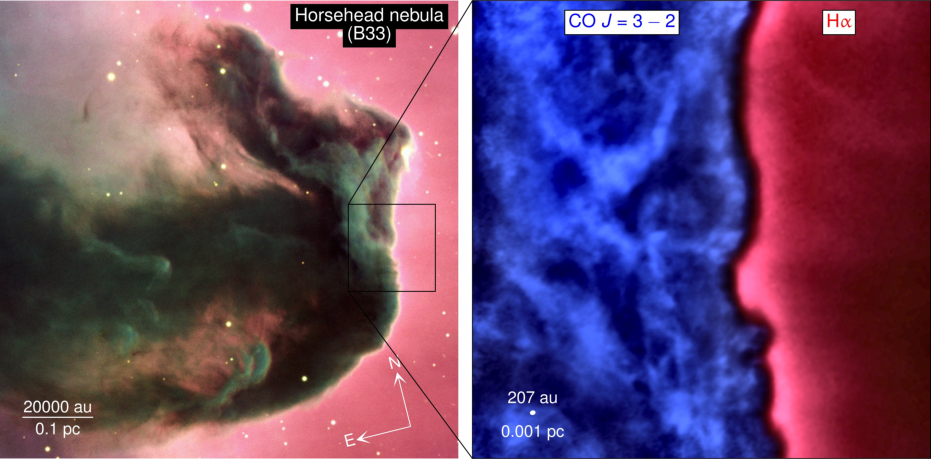
\includegraphics[width=.8\textwidth]{horsehead_HernandezVera2023.pdf}
        \begin{overpic}[width=.8\textwidth]{horsehead_HernandezVera2023.pdf}
            \put(70, -3){\scriptsize Credit: Hernández-Vera et al. 2023}
        \end{overpic}
    \end{center}
    \begin{itemize}
        % \item \(\sim \qty{400}{pc}\) from us
        \item observed \textbf{edge-on} $\Rightarrow$  observational access to the chemical stratification
    \end{itemize}
    \vfill
    part of a collaboration between JPL, Paris Observatory, IRAM, and CSIC Madrid to study the presence of water in the Horsehead Nebula\par
    \qt{This project is part of a collaboration between JPL (Darek Lis), Paris Observatory (us), IRAM (David Teyssier), and CSIC Madrid (Javier Goicoechea) to study the presence of water in the Horsehead Nebula. More generally, we aim to explain the localization of several emission lines, including \ce{H2O}, \ce{C}, \ce{^{12}CO}, \ce{^{13}CO}, and \ce{^{18}CO} in the Horsehead.}
\end{frame}

\section{Data}
\begin{frame}{Data}
    % \centering
    % \vskip-0.6em\resizebox{.88\textwidth}{!}{
    %     \begin{tabular}{cclll}
    %         \midrule
    %         \midrule
    %         Notation & Species & Upper Level & Lower Level & Frequency (\unit{GHz}) \\
    %         \midrule
    %         \ce{H2O}            & \ce{H2O}  & J=1, Ka=1, Kc=0 & J=1, Ka=0, Kc=1 & 557.30 \\
    %         \ce{C[II]}          & \ce{C+}   & 2P J=3/2 & 2P J=1/2 & 1902.59 \\
    %         \ce{C[I]}           & \ce{C}    & 3P J=1 & 3P J=0 & 492.02 \\
    %         \ce{CO} (2-1)       & \ce{CO}   & v=0, J=2 & v=0, J=1 & 230.538 \\
    %         \ce{CO} (4-3)       & \ce{CO}   & v=0, J=4 & v=0, J=3 & 461.041 \\
    %         % \ce{^{13}CO} (2-1)  & \ce{^{13}CO} & v=0, J=2 & v=0, J=1 & 220.399 \\
    %         \ce{C^{18}O} (2-1)  & \ce{C^{18}O} & v=0, J=2 & v=0, J=1 & 219.560 \\
    %         \midrule
    %         \bottomrule
    %     \end{tabular}}
    % \vfill
    \begin{columns}
        \begin{column}{.25\textwidth}
            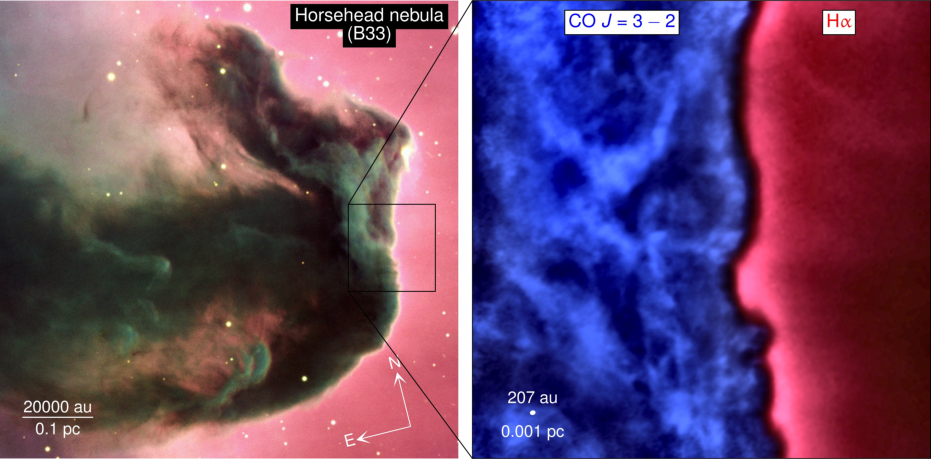
\includegraphics[width=\textwidth,trim=100 0 225 0,clip,keepaspectratio]{horsehead_HernandezVera2023.pdf}
        \end{column}
        \begin{column}{.75\textwidth}
            observations along a cut through the Horsehead Nebula\par
            \hskip1em \textbullet\hskip0.7em \ce{C+}, \ce{C}, \ce{CO} and its isotopologues, and \ce{H2O}\vskip1em
            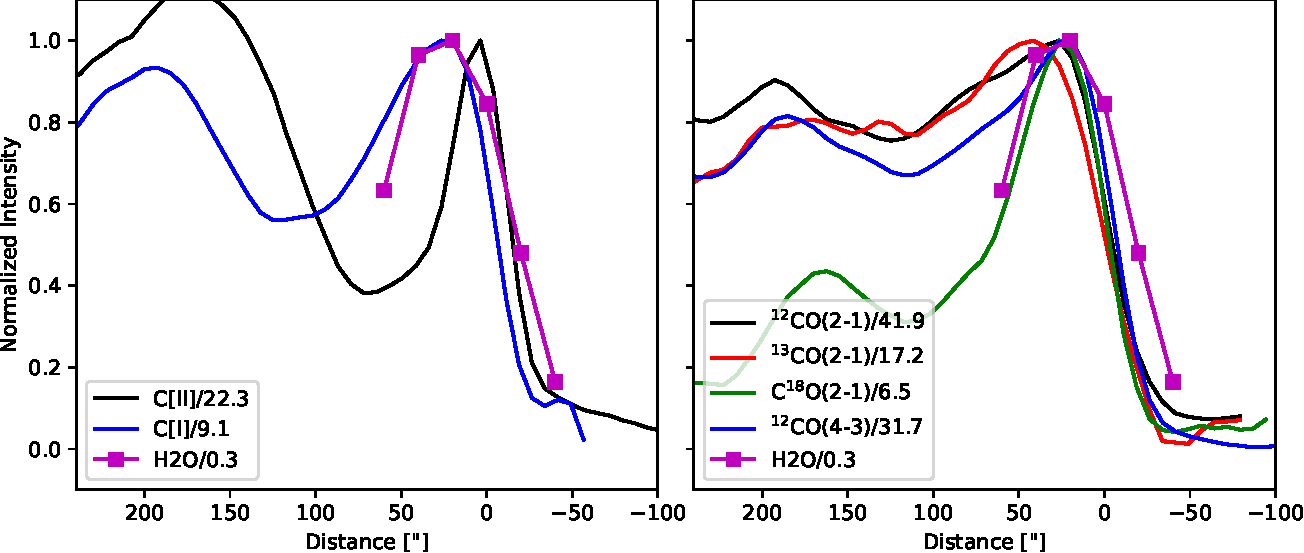
\includegraphics[width=\textwidth,keepaspectratio]{observed_lines.pdf}
        \end{column}
    \end{columns}
\end{frame}

\section{Motivation}
\begin{frame}[t]{Motivation}
    \begin{minipage}[t][.32\textheight][t]{\textwidth}
        \vskip-1.2em\textbf{1D PDR models}
        \begin{itemize}
            \setlength{\itemsep}{0pt} 
            \item infinite and uniform in two dimensions, depth-dependent only\par
            \hskip1em $\Rightarrow$ allows for a detailed study of the physical and chemical processes\qt{This is a good approximation of the physics as the physical properties of the cloud are largely dependent on the UV field}
            \item cannot be compared directly to edge-on observations \qt{As mentioned in the last slides, edge-on observations provide insights into the chemical stratification of PDRs.}
        \end{itemize}
        \only<2->{\textbf{Proposed Solution:}
        \begin{itemize}
            \setlength{\itemsep}{0pt} 
            \item approximate edge-on regions with \textbf{curvature radius}.
            \item a spherical geometry wrapper for the \mdpdr{} code
            % \begin{itemize}
            %     \item Compute spatial profiles of \textbf{column densities}.
            %     \item Solve \textbf{radiative transfer} for line intensities.
            % \end{itemize}
            % \item \textbf{Case Study: Horsehead Nebula}—ideal testbed with tracer emission data.
        \end{itemize}}
    \end{minipage}
    \vfill
    \begin{columns}[T]
        \begin{column}{.4\textwidth}
            \centering
            \only<-2>{\vskip0.5em
            % 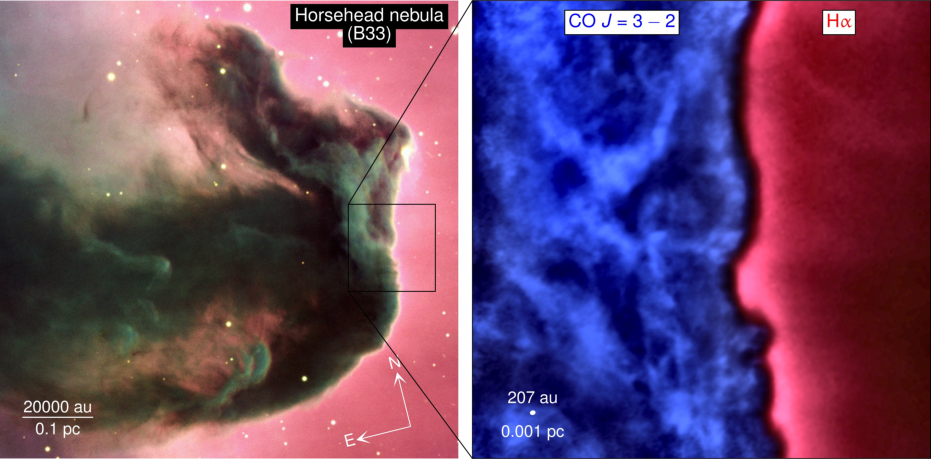
\includegraphics[width=.8\textwidth,angle=180,trim=0 0 225 0,clip,keepaspectratio]{horsehead_HernandezVera2023.pdf}
            \begin{overpic}[width=.85\textwidth,angle=180,trim=0 0 225 0,clip,keepaspectratio]{horsehead_HernandezVera2023.pdf}
                \only<2>{\put(14, 37){
\begin{tikzpicture}
                    \draw [-, line width=3pt, Orchid] (0, 0) arc[start angle=90, end angle=270, radius=1];
                \end{tikzpicture}}}
            \end{overpic}
            }
            \only<3>{\hskip2em\begin{itemize}
                \item spatial profiles of \textbf{column densities}
                \item solve \textbf{radiative transfer} for line intensities
                \item \textbf{convolution} with the instrument resolution
            \end{itemize}}
        \end{column}
        \begin{column}{.48\textwidth}
            \includegraphics<1->[width=.49\textwidth,height=.58\textheight,keepaspectratio]{slab_geometry.pdf}
            \includegraphics<2->[width=.49\textwidth,height=.58\textheight,keepaspectratio]{slab_to_sphere.pdf}
        \end{column}
    \end{columns}
\end{frame}

\section{Methods}
\subsection{The \mdpdr{} Code}
\begin{frame}[t]{The \mdpdr{} Code}
    % stationary 1D PDR code\par
    % \textbullet\hskip0.7em radiative transfer (line and continuum in the UV)\par
    % \textbullet\hskip0.7em chemical balance\hskip1em \textbullet\hskip0.7em level populations\hskip1em \textbullet\hskip0.7em thermal balance\par\vskip1em
    \begin{columns}
        \begin{column}{.6\textwidth}
            stationary 1D PDR code
            {\small \begin{itemize}
                \item radiative transfer\hskip1em \textbullet\hskip.7em chemical balance
                \item level populations \hskip1em \textbullet\hskip.7em thermal balance
            \end{itemize}}
        \end{column}
        \begin{column}{.4\textwidth}
            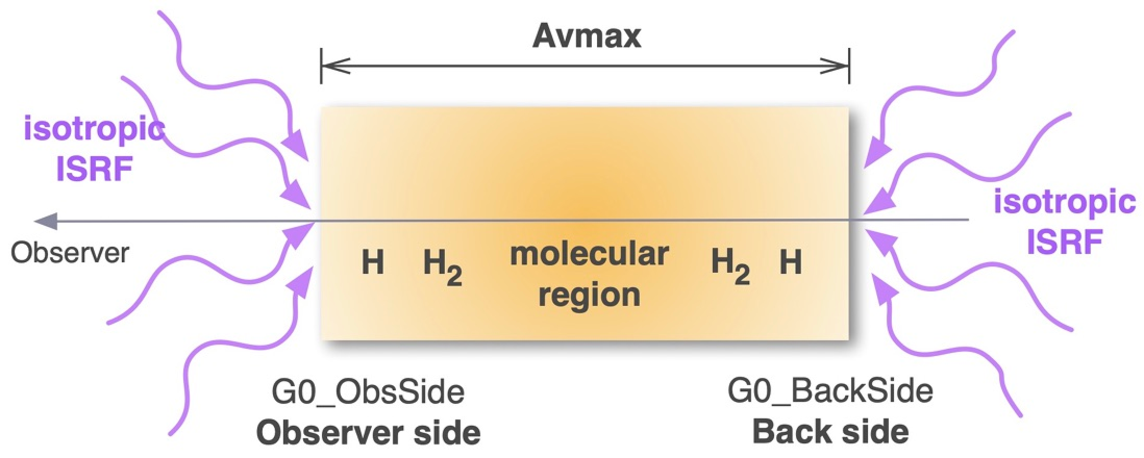
\includegraphics[width=\textwidth,keepaspectratio]{schemePDR.pdf}
        \end{column}
    \end{columns}
    \qt{In a complex model such as the MeudonPDR code, different levels or types of approximations are possible}
    % \centering
    % \resizebox{.8\textwidth}{!}{
    %     \begin{tabular}{ll}
    %         \midrule
    %         \midrule
    %         Cloud size ($A_{V, \max}$) & 40 \\
    %         Proton density ($n_H$) & \qtyrange[range-units=single,range-phrase=~--~]{3e4}{3e6}{cm^{-3}}\\
    %         Pressure ($P$) & \qtyrange[range-units=single,range-phrase=~--~]{1e6}{1e7}{K\,cm^{-3}} \\
    %         ISRF & shape: Mathis, geometry: beam\_isot \\
    %         ISRF scaling factor & $G_0^\mr{obs} = 100,\ G_0^\mr{back} = 0.04$\\
    %         UV radiative transfer method & FGK approximation, or\\
    %         & exact \ce{H2} self- and mutual shielding \\
    %         Turbulent velocity dispersion & \qty{2}{\km\per\second} \\
    %         Extinction Curve & HD38087\\
    %         $R_V = A_V / E(B-V)$ & $5.50$ \\
    %         $C_D = N_H / E(B-V)$ & $1.57\times 10^{22}$\\
    %         \bottomrule
    %     \end{tabular}
    % }
    % \vfill
    % $\Rightarrow P = \qty{5e6}{K\,cm^{-3}}$ + \ce{H2} radiative transfer + surface chemistry
    \centering
    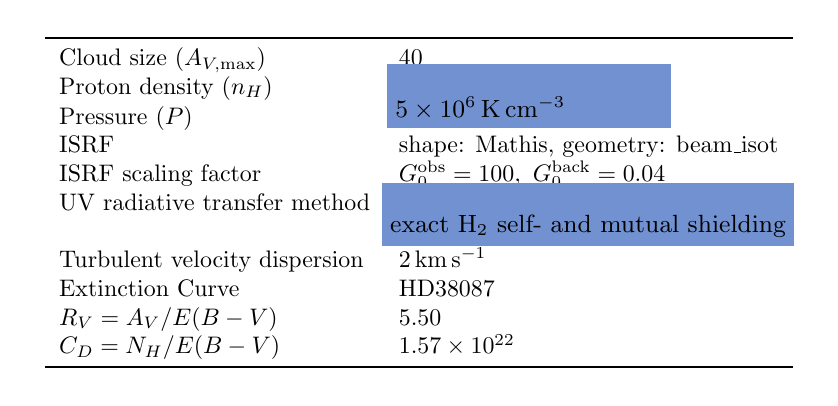
\begin{tikzpicture}
        \node (table) at (0, 0) {
            \resizebox{.8\textwidth}{!}{
                \begin{tabular}{ll}
                    \toprule
                    Cloud size ($A_{V, \max}$) & 40 \\
                    Proton density ($n_H$) & \qtyrange[range-units=single,range-phrase=~--~]{3e4}{3e6}{cm^{-3}}\\
                    Pressure ($P$) & \qtyrange[range-units=single,range-phrase=~--~]{1e6}{1e7}{K\,cm^{-3}} \\
                    ISRF & shape: Mathis, geometry: beam\_isot \\
                    ISRF scaling factor & $G_0^\mr{obs} = 100,\ G_0^\mr{back} = 0.04$\\
                    UV radiative transfer method & FGK approximation, or\\
                    & exact \ce{H2} self- and mutual shielding \\
                    Turbulent velocity dispersion & \qty{2}{\km\per\second} \\
                    Extinction Curve & HD38087\\
                    $R_V = A_V / E(B-V)$ & $5.50$ \\
                    $C_D = N_H / E(B-V)$ & $1.57\times 10^{22}$\\
                    \bottomrule
                \end{tabular}
            }
        };
        \only<2>{\node at (1.4, 1.5) {\colorbox{PSL_shade}{\small\phantom{\qty{5e6}{K\,cm^{-3}}1\unit{{K\,cm^{-3}}}}}}; 
        \node at (1.4, 1.2) {\colorbox{PSL_shade}{\small\qty{5e6}{K\,cm^{-3}}\phantom{1\unit{{K\,cm^{-3}}}}}}; 
        \node at (2.15, 0) {\colorbox{PSL_shade}{\small\phantom{exact \ce{H2} self- and mutual shielding}}}; 
        \node at (2.15, -0.3) {\colorbox{PSL_shade}{\small exact \ce{H2} self- and mutual shielding}};}

        % % Draw shapes or highlight areas (e.g., rectangle around a row)
        % \draw[thick, orange, rounded corners] (-3.8, 0.5) rectangle (3.8, 1.2); % Highlight region
    \end{tikzpicture}
    \only<2>{
        \colorbox{PSL_shade}{+ surface chemistry}
    }
    \footnotetext{Parameter values are based on Maillard, 2023}
\end{frame}

% \section{Convolved Column Densities in a Spherical PDR}
\subsection{Column Densities in a Spherical PDR}
\begin{frame}{From Slab to Spherical Geometry}
    % \centering
    % 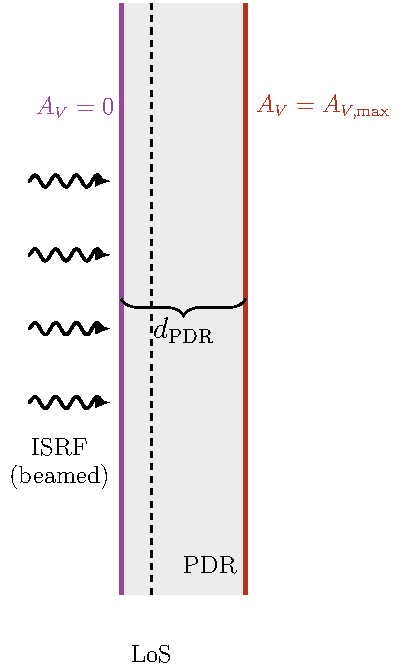
\includegraphics[width=.3\textwidth,height=.6\textheight,keepaspectratio]{slab_geometry.pdf}
    % 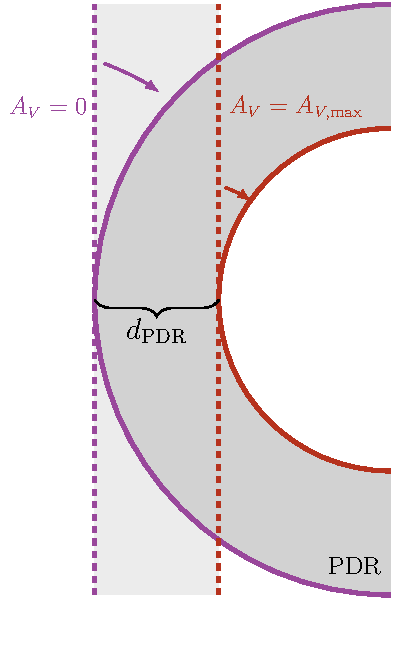
\includegraphics[width=.32\textwidth,height=.6\textheight,keepaspectratio]{slab_to_sphere.pdf}
    % 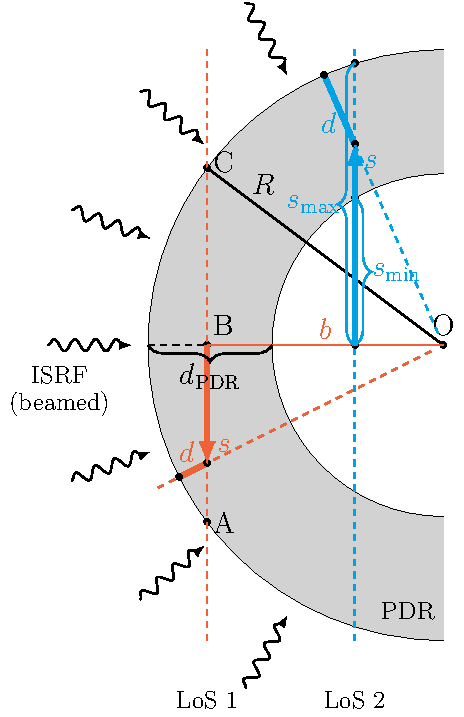
\includegraphics[width=.38\textwidth,height=.64\textheight,keepaspectratio]{sphere_geometry.pdf}
    \begin{columns}[T]
        \begin{column}{.6\textwidth}
            % \only<1>{\vfill
            % 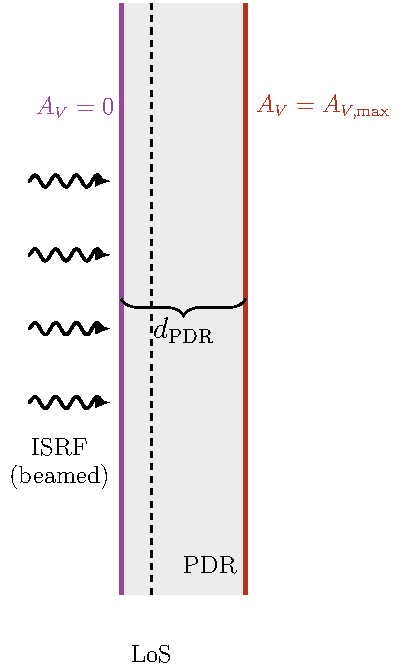
\includegraphics[width=.5\textwidth,height=.6\textheight,keepaspectratio]{slab_geometry.pdf}
            % 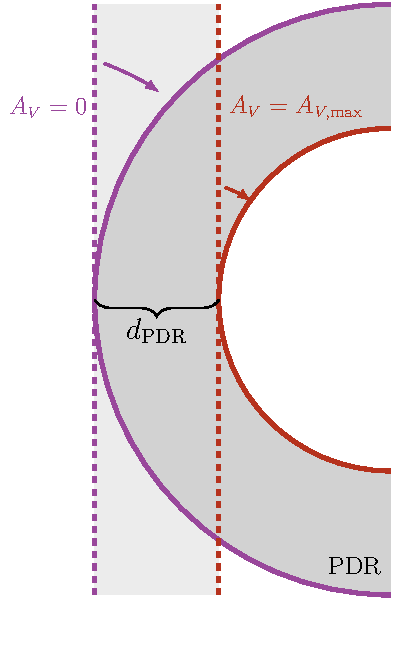
\includegraphics[width=.5\textwidth,height=.6\textheight,keepaspectratio]{slab_to_sphere.pdf}
            % \vfill}
            \only<1>{
            Input: \begin{itemize}
                \item level number density $n_X(d)$
                \item cloud radius $R$ (free parameter)
                \item LoS impact parameter $b$
            \end{itemize}
            Algorithm:
            \begin{itemize}
                \item interpolation of $n_X(d) = f(d)$ to allow computation of $n_X$ at any depth
                % \item depth along LoS, $s_{\min}, s_{\max}$ from geometry
                % \resizebox{\textwidth}{!}{%
                %     \begin{minipage}{\textwidth}
                %         \begin{align*}
                %             &s_{\max} = \sqrt{R^2 - b^2}\\
                %             &s_{\min} = \left\{\begin{array}{ll}
                %                 0  &  b > R - d_\mr{PDR} \\
                %                 \sqrt{(R - d_\mr{PDR})^2 - b^2}  &  b < R - d_\mr{PDR}
                %             \end{array}\right.
                %         \end{align*}
                %     \end{minipage}  
                % }
                % \item \(d = R - \sqrt{s^2 + b^2} \Rightarrow n_X(s)\)
                \item \(d = R - \sqrt{s^2 + b^2} \Rightarrow n_X(s)\)
                % \(\Rightarrow n_X(s) = n_X(R - \sqrt{s^2 + b^2})\)
                \item integrate along the LoS
                \begin{equation*}
                    N_X(b) = 2\int_{0}^{s_{\max}} n_X(s') \dd{s'}
                \end{equation*}
            \end{itemize}
            For optically thin lines, $I_\nu \propto N_X$}
        \end{column}
        \begin{column}{.32\textwidth}
            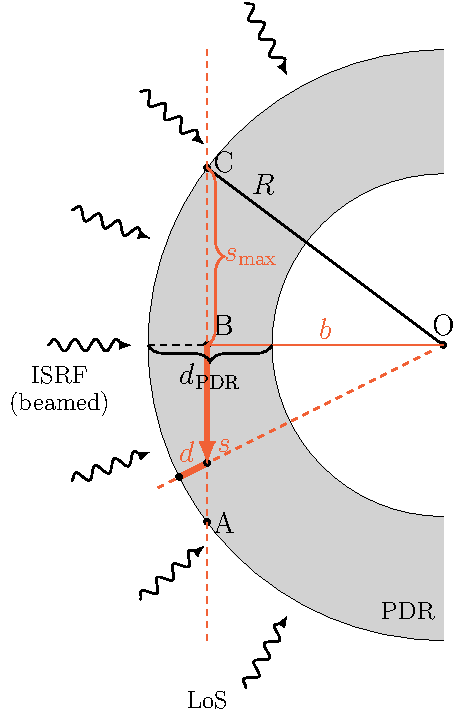
\includegraphics[width=\textwidth,keepaspectratio]{sphere_geometry_1LoS.pdf}
        \end{column}
    \end{columns}
\end{frame}

\subsection{Convolution with the Instrument Resolution}
\begin{frame}[t]{Convolution with the Instrument Resolution}
    \begin{columns}
        \begin{column}{\textwidth}
            Algorithm
            \begin{itemize}
                \item<1-> interpolate the model grids to uniform ones \mintinline{python}{x_uniform}, \mintinline{python}{y_uniform} 
                \item<2-> Gaussian kernel with the given resolution, full width half maximum (FWHM)
                \begin{equation*}
                    \sigma = \text{FWHM}\,/\,(2\sqrt{2 \ln 2}),\ g(x) = \frac{1}{\sigma\sqrt{2\pi}}\exp(-\frac{x^2}{2\sigma^2})
                \end{equation*}
                \item<4-> convolution with truncation at $3\sigma$, padding \mintinline{python}{y_uniform} with 0
                % \begin{equation*}
                %     (f * g) (x) = \frac{1}{K} \sum_{\tau = x_{\min} - 3\sigma}^{x_{\max} + 3\sigma}F(\tau)g(x - \tau)\Delta x
                % \end{equation*}
            \end{itemize}
        \end{column}
        % \begin{column}{.3\textwidth}
            % \includegraphics<1>[width=\textwidth,keepaspectratio]{convv_process_1.pdf}
            % \includegraphics<2>[width=\textwidth,keepaspectratio]{convv_process_2.pdf}
            % \includegraphics<3->[width=\textwidth,keepaspectratio]{convv_process_3.pdf}
        % \end{column}
    \end{columns}
    \vfill\centering
    \includegraphics<4>[width=.8\textwidth,keepaspectratio]{convolution_co21.pdf}
\end{frame}

% \begin{frame}[t]{Convolved Column Densities from Spherical Models}
%     slab vs spherical geometry
%     \begin{center}
%         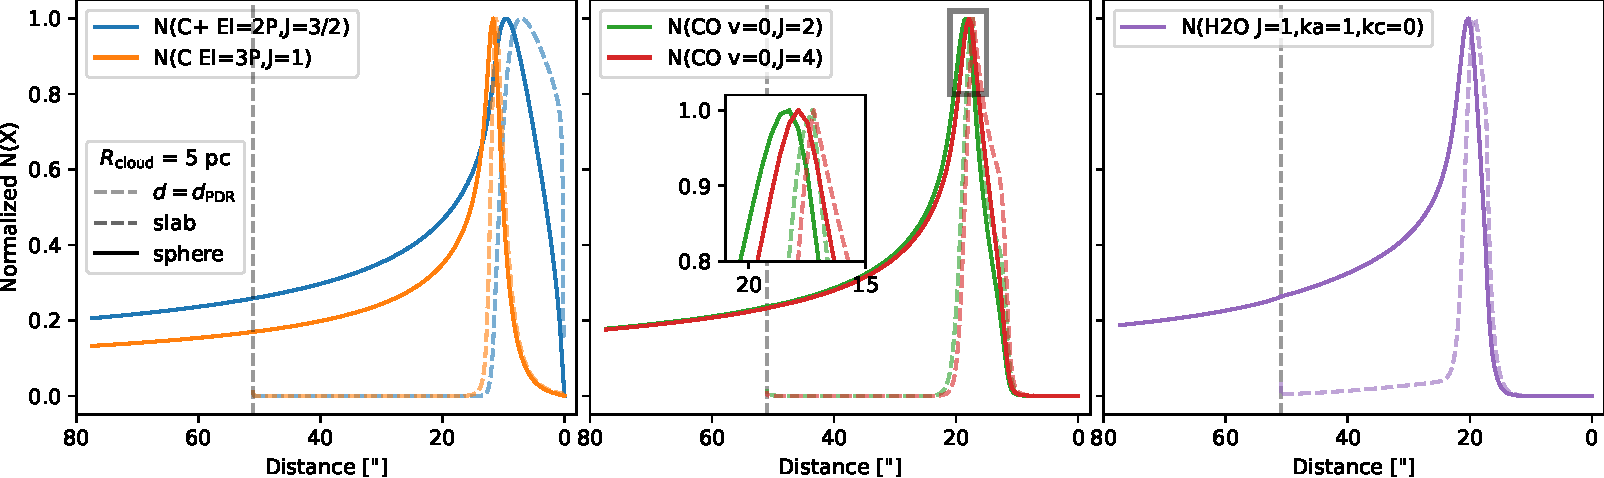
\includegraphics[width=.88\textwidth,keepaspectratio]{column_densities.pdf}
%     \end{center}
% \end{frame}

% \begin{frame}
%     \begin{columns}
%         \begin{column}{.35\textwidth}
%             \centering
%             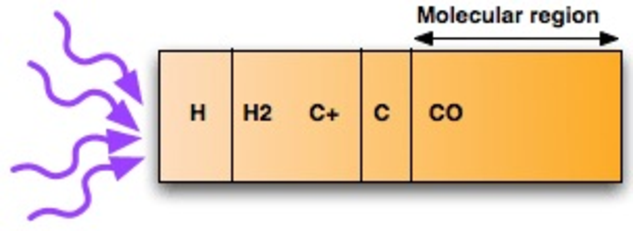
\includegraphics[width=\textwidth,keepaspectratio]{Schema_PDR.pdf}
%             \hfill\includegraphics[width=.7\textwidth,keepaspectratio]{geometry_2LoS.pdf}
%             NB: radiation from the left side
%         \end{column}
%         \begin{column}{.65\textwidth}
%             \only<1>{Input
%             \begin{itemize}
%                 \item $n_X(d)$ computed by the MeudonPDR code
%                 \item radius of the fictitious spherical cloud, $R$
%                 \item each LoS is parametrized by a given $b$
%             \end{itemize}}
%             \only<2>{algorithm
%             \begin{itemize}
%                 \item interpolation of $n_X(d) = f(d)$ to allow computation of $n_X$ at any depth
%                 \item the range of distances along LoS inside the cloud
%                 \begin{align*}
%                     &s_{\max} = \sqrt{R^2 - b^2},\\
%                     &s_{\min} = \left\{\begin{array}{ll}
%                        0  &  b > R - d_\mr{PDR} \\
%                        \sqrt{(R - d_\mr{PDR})^2 - b^2}  &  b < R - d_\mr{PDR}
%                     \end{array}\right.
%                \end{align*}
%                \item from geometry, $d = R - \sqrt{s^2 + b^2}$, therefore
%                \begin{equation*}
%                     n_X(s) = f(R - \sqrt{s^2 + b^2})
%                \end{equation*}
%                \item integrate along the LoS to get the column densities
%                \begin{equation*}
%                     N_X(b) = 2\int_{s_{\min}}^{s_{\max}} n_X(s') \dd{s'}
%                \end{equation*}
%             \end{itemize}}
%         \end{column}
%     \end{columns}
% \end{frame}

\section{Results}
\subsection{Convolved Column Densities from Spherical Models}
\begin{frame}[t]{Convolved Column Densities from Spherical Models}
    \vskip-0.8em step 1: slab vs spherical geometry
    \begin{center}
        % 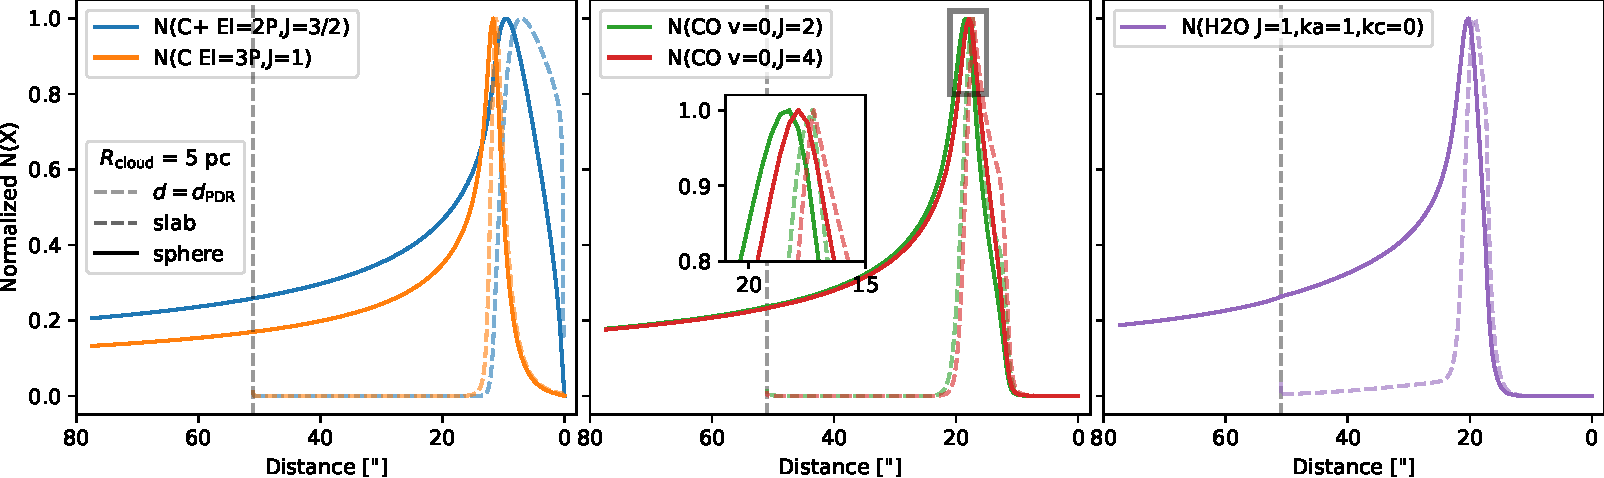
\includegraphics[width=.88\textwidth,keepaspectratio]{column_densities.pdf}
        \begin{overpic}[width=.88\textwidth,keepaspectratio]{column_densities.pdf}
            \only<2->{
                \put(-7, 32){\colorbox{PSL_shade}{spherical geometry: the peaks shift to deeper locations within the cloud}}
            }
        \end{overpic}
    \end{center}
    \only<3->{\vskip-0.5em step 2: convolved vs unconvolved column densities
    \begin{center}
        % \includegraphics<3>[width=.9\textwidth,keepaspectratio]{convolved_column_densities_arcsec.pdf}
        \begin{overpic}[width=.9\textwidth,keepaspectratio]{convolved_column_densities_arcsec.pdf}
            \only<4>{
                \put(-7, 32){\colorbox{PSL_shade}{convolution: line spatial profiles are smoothed and further extended}}
            }
        \end{overpic}
    \end{center}}
\end{frame}

\begin{frame}[t]{Compare Column Densities with Observations}
    \textbf{convolved column densities} from \textbf{spherical models} match observations better\vskip1em
    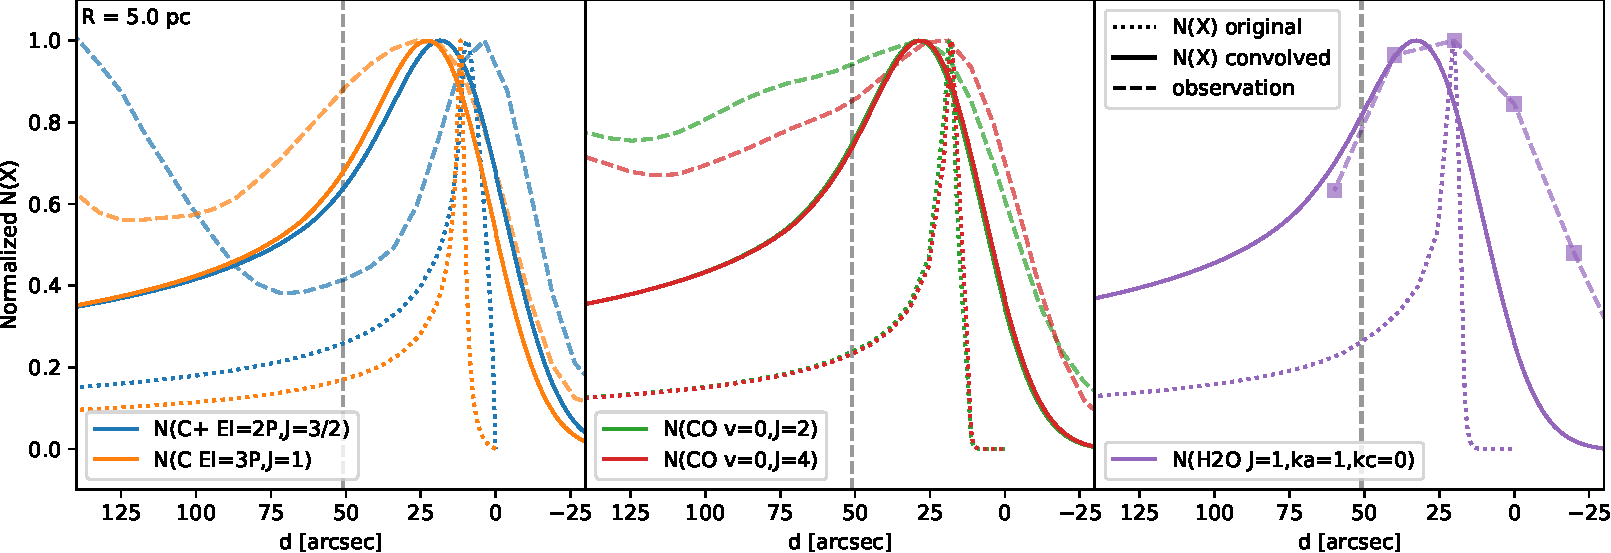
\includegraphics[width=\textwidth,keepaspectratio]{colden_Rcloud5pc.pdf}
    \vskip2em
    \only<2->{profile width $\checkmark$, shape on the front side $\checkmark$, shape on the back side $\times$\par\vskip.5em}
    \only<3>{Can cloud radius make a difference?}
\end{frame}

\subsection{Effect of Cloud Radius on Column Densities}
\begin{frame}[t]
    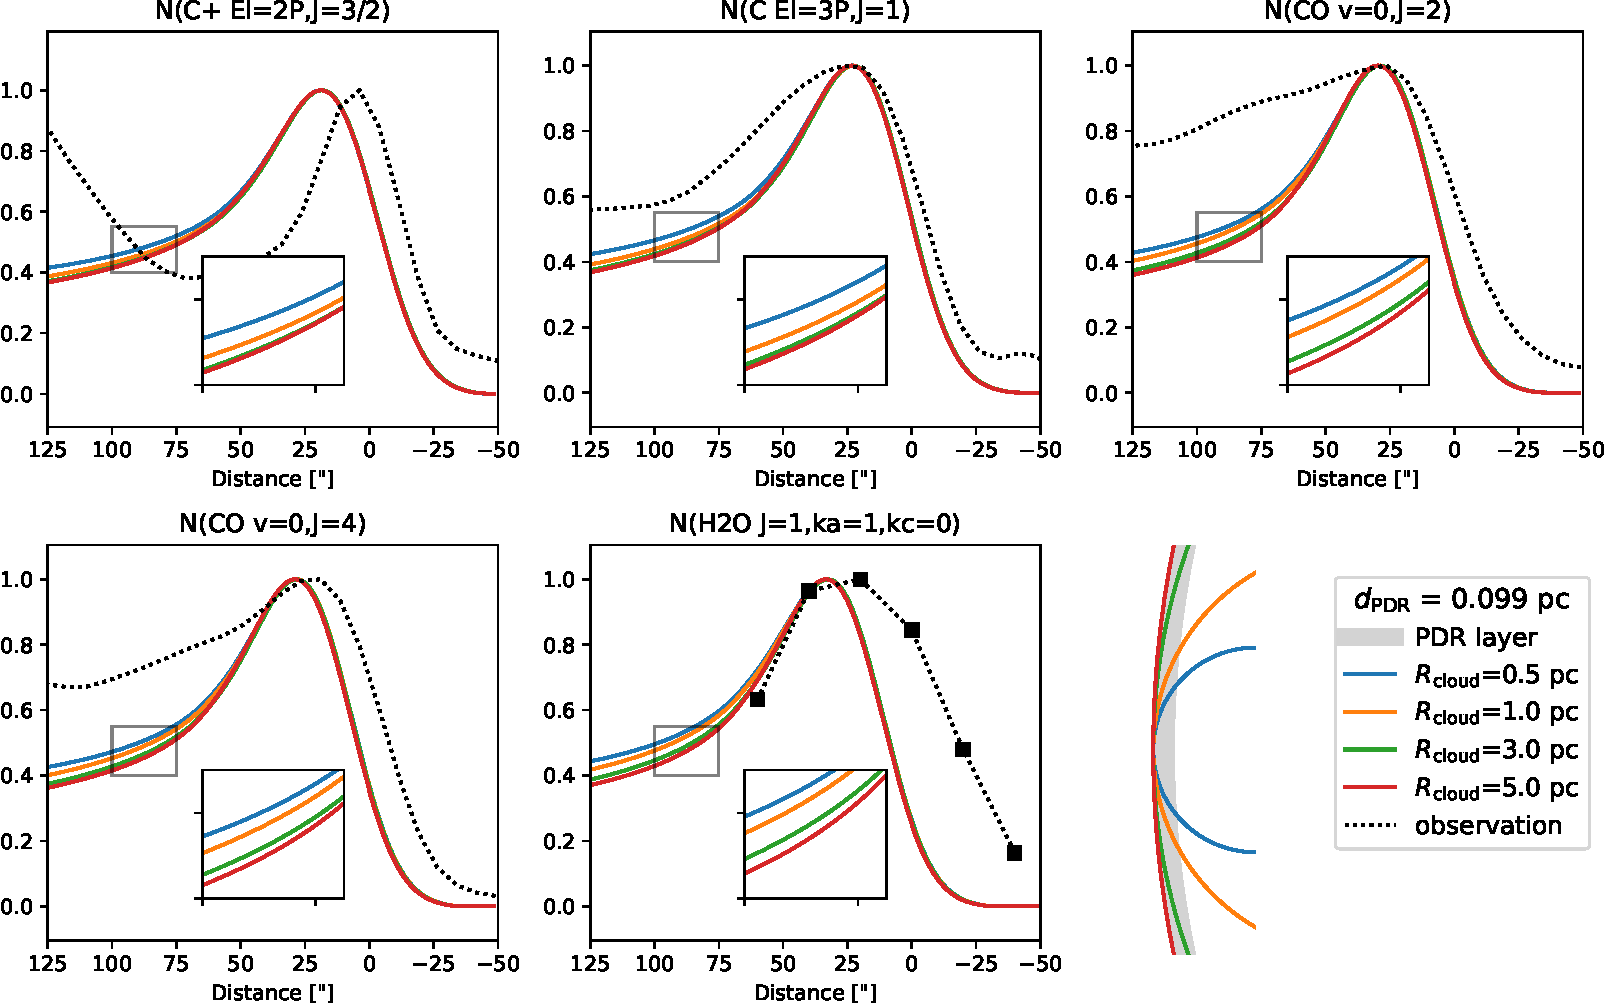
\includegraphics[width=\textwidth,keepaspectratio]{comp_cloud_radius.pdf}
    \only<2->{\colorbox{PSL_shade}{The differences in column density profiles are trivial} 
    \only<3>{\phantom{$\Rightarrow$} \parbox{.3\textwidth}{Tail shape $\times, I_\nu \not\propto N_X$?}}
    \only<4>{$\Rightarrow$ \parbox{.3\textwidth}{need to solve the radiative transfer equation}}}
\end{frame}

\section{Solving the Radiative Transfer Equation along LoS}
\begin{frame}[t]{Solving the Radiative Transfer Equation along LoS}
    The radiative transfer equation (neglecting dusts, scattering)
    \begin{equation*}
        \fird[I_\nu]{s} = A_{ul} n_u\frac{h\nu}{4\pi}\phi(\nu) +  B_{ul} n_u\frac{h\nu}{4\pi}I_\nu \phi(\nu) -  B_{lu} n_l\frac{h\nu}{4\pi}I_\nu \phi(\nu), \label{eq:rte}
    \end{equation*} 
    with a thermal and turbulent broadening line profile $\phi(\nu)$\par\vskip1em
    % \begin{equation*}
    %     \phi(\nu) = \frac{1}{\sqrt{\pi} \Delta\nu_D} \exp\left(-\frac{(\nu - \nu_0)^2}{\Delta\nu_D^2}\right)
    % \end{equation*}
    \only<2>{For a toy problem with constant lower and uppper level populations
    \begin{equation*}
        \fird[I_\nu]{s} = c_1  + c_2 I_\nu, \text{ with } c_1, c_2 \text{ constants}
    \end{equation*} 
    \centering
    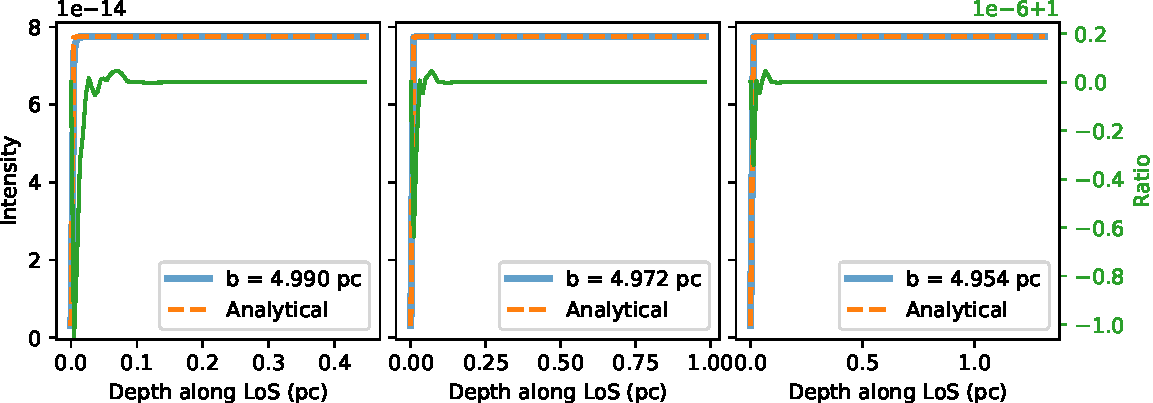
\includegraphics[width=.88\textwidth,keepaspectratio]{rte_constant_density.pdf}}
\end{frame}

% \subsection{Line Profiles with Radiative Transfer}

\begin{frame}{Conclusions}
    \mdpdr{} wrapper
    \begin{itemize}
        \item \textbf{column densities in spherical geometry}\par
        \only<1>{\phantom{\hskip1em $\Rightarrow$ extended profiles with peaks shifted to greater depths}}
        \only<2->{\hskip1em $\Rightarrow$ extended profiles with peaks shifted to greater depths}
        \item \textbf{convolution with the instrument resolution}\par
        \only<-2>{\phantom{\hskip1em $\Rightarrow$ further smooths and extends the line spatial profiles}}
        \only<3->{\hskip1em $\Rightarrow$ further smooths and extends the line spatial profiles}
        \item \textbf{comparison with observations}\par
        \only<-3>{\phantom{\hskip1em $\Rightarrow$ convolved column density profiles match the observation better}\par
        \phantom{\hskip1em $\Rightarrow$ cloud radius has a trivial effect}}
        \only<4->{\hskip1em $\Rightarrow$ convolved column density profiles match the observation better\par
        \hskip1em \phantom{$\Rightarrow$} cloud radius has a trivial effect\par}
        \only<-4>{\phantom{radiative transfer equation needs to be solved}}
        \only<5->{radiative transfer equation needs to be solved}
        \item \textcolor{lightgray}{radiative transfer for line intensities}
        \begin{itemize}
            \item<6-> solver for the radiative transfer equation
            \item<6-> preliminary results at the line centers
            \item<7> \textcolor{lightgray}{full solution with line broadening}
        \end{itemize}
    \end{itemize}

\end{frame}

{
% \setbeamercolor{background canvas}{bg=PSL_shade!20!white}
\usebackgroundtemplate{
    \tikz\node[opacity=0.6, at=(current page.center)]{
        \hskip-0.4em
        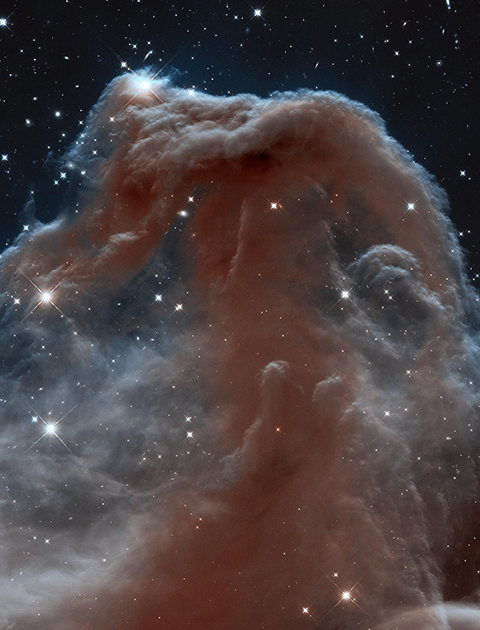
\includegraphics[width=\paperwidth,keepaspectratio]{horsehead_hst.png}};
}
\begin{frame}[label=toc]{Thank you!}
    \begin{columns}[T]
        \begin{column}{.1\textwidth}
        \end{column}
        \begin{column}{.9\textwidth}
            \tableofcontents
        \end{column}
        % \begin{column}{.1\textwidth}
        % \end{column}
    \end{columns}
    \vskip1em
    \centering\colorbox{PSL_dark}{\textcolor{white}{Questions?}}
\end{frame}}

\backupbegin

\begin{frame}{Mutiple Peaks in the Observed Profiles}
    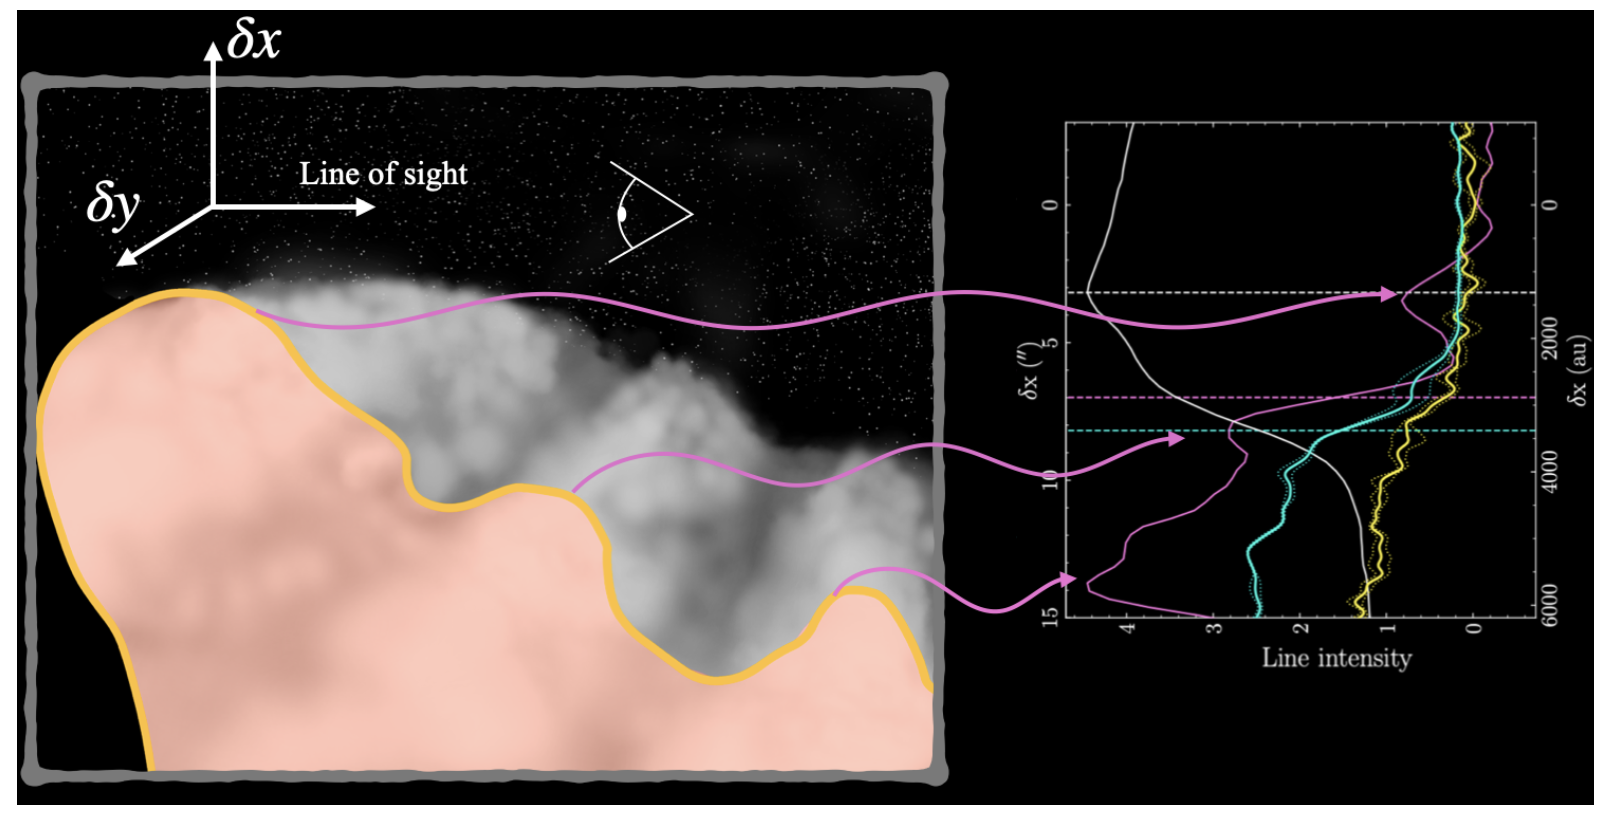
\includegraphics[width=\textwidth,keepaspectratio]{multiple_fronts.png}
    \hfill\scriptsize Credit: Maillard, 2023
\end{frame}

\begin{frame}{Exact H2 Self- and Mutual Shielding}
    \centering
    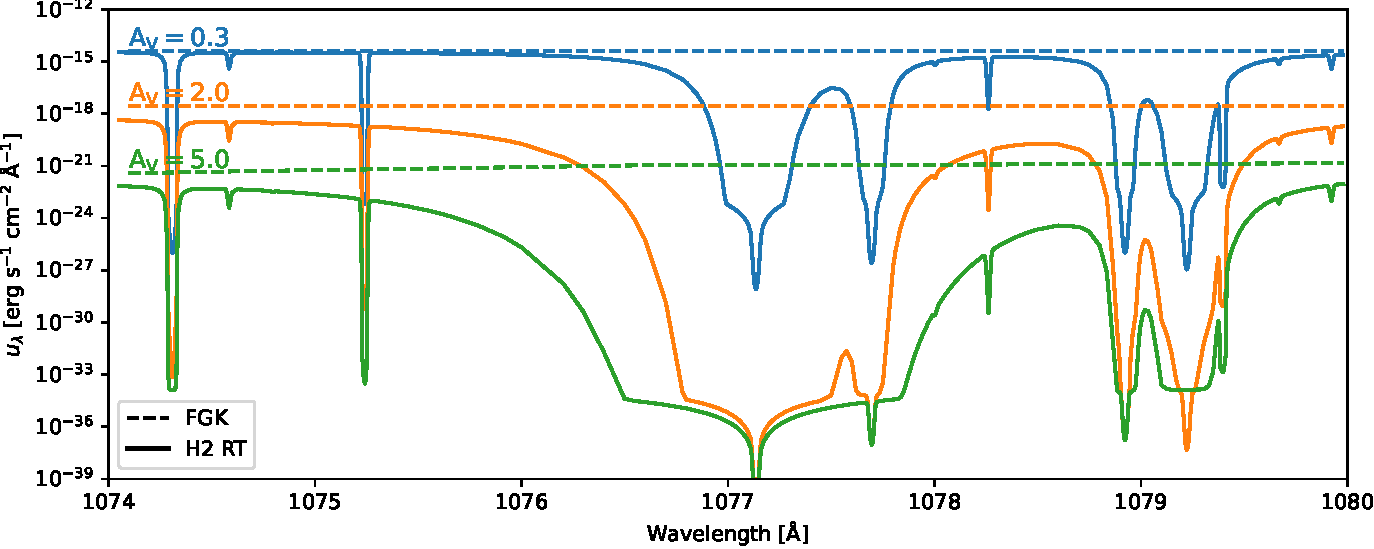
\includegraphics[width=.8\textwidth,keepaspectratio]{spectra_fgkh2_1.pdf}
\end{frame}

\begin{frame}{Exact H2 Self- and Mutual Shielding 2}
    \centering
    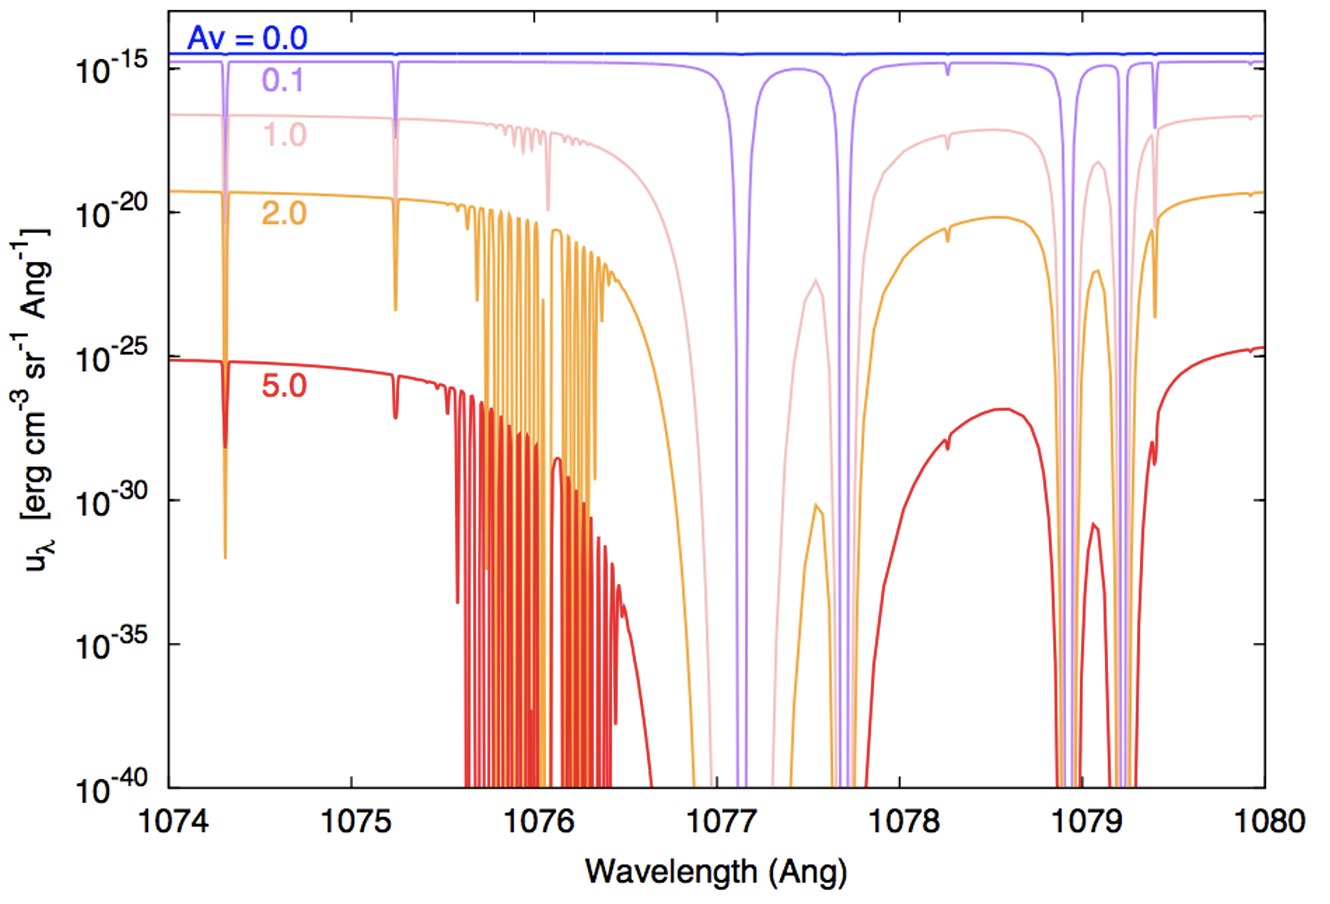
\includegraphics[width=.88\textwidth,keepaspectratio]{localenergydensity.png}
\end{frame}

\begin{frame}{Preliminary results of solving RTE at the line centers}
    \centering
    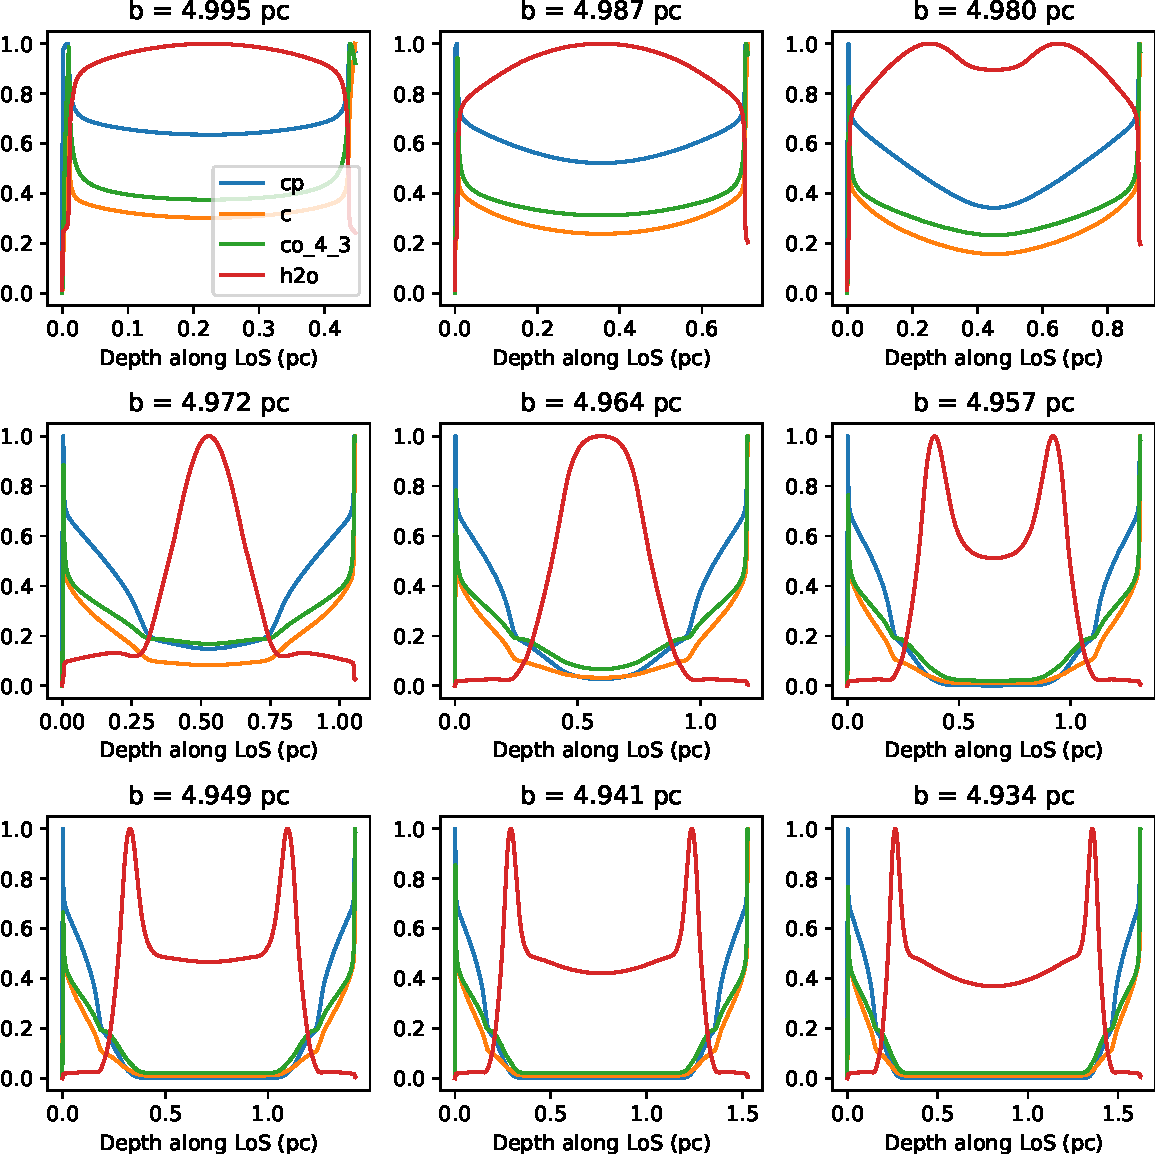
\includegraphics[width=\textwidth,height=.85\textheight,keepaspectratio]{rte_comparison.pdf}
\end{frame}

\backupend

\end{document}